
\begin{figure}
  \centering
  \begin{tabular}{p{50mm}p{50mm}p{50mm}}
    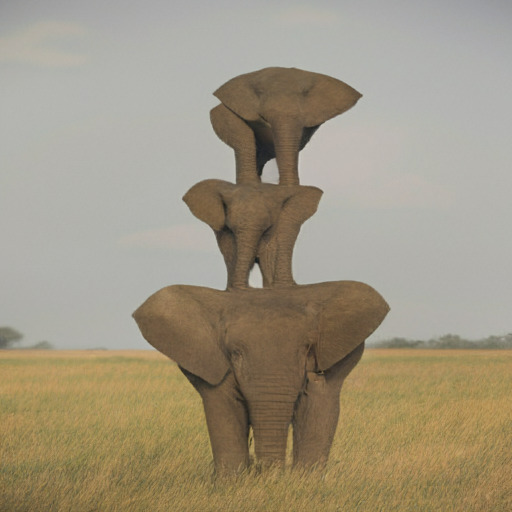
\includegraphics[width=50mm]{figs/verticals/cardinality_00430_maskgit_sresg1r1} &
    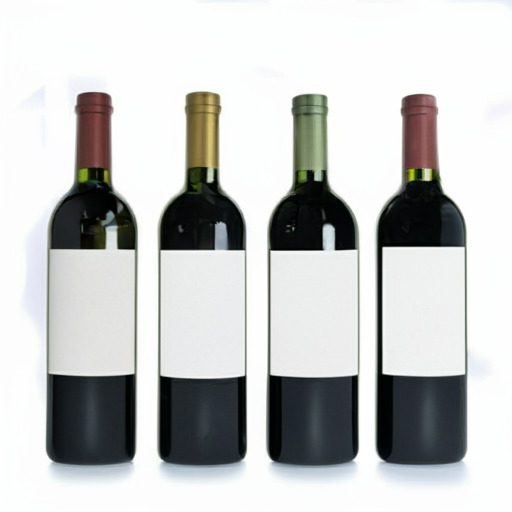
\includegraphics[width=50mm]{figs/verticals/cardinality_00708_maskgit_sresg1r1} &
    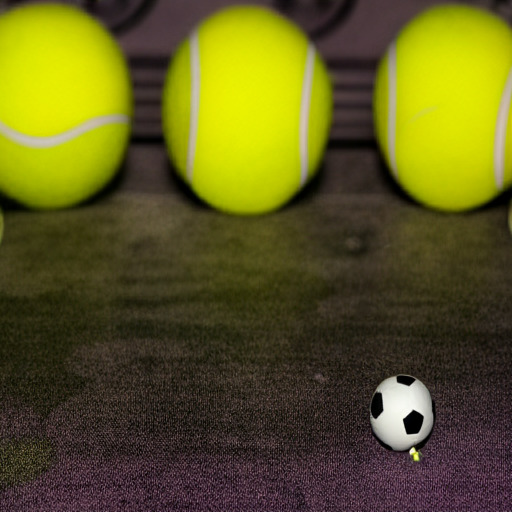
\includegraphics[width=50mm]{figs/verticals/cardinality_00087_maskgit_sresg1r1}
    \\
    \small Three elephants standing on top of each other. &
    \small Four wine bottles. &
    \small A tiny football in front of three yellow tennis balls.
    \\
    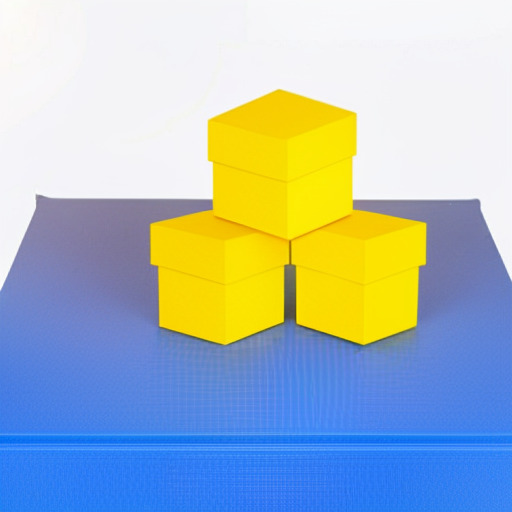
\includegraphics[width=50mm]{figs/verticals/composition_00678_maskgit_sresg1r1} &
    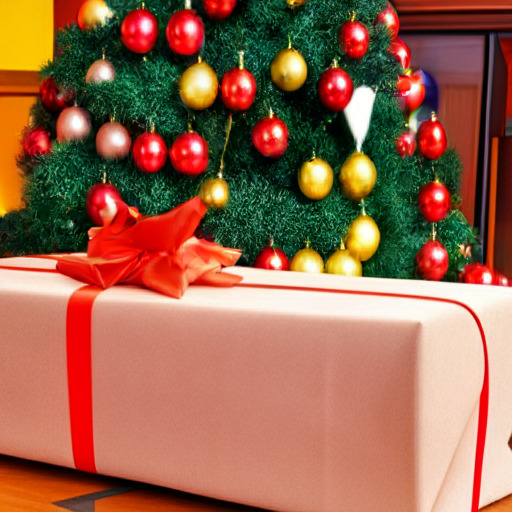
\includegraphics[width=50mm]{figs/verticals/composition_00681_maskgit_sresg1r1} &
    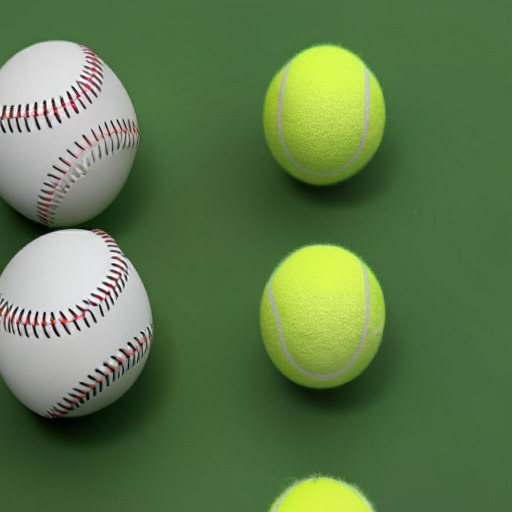
\includegraphics[width=50mm]{figs/verticals/composition_01426_maskgit_sresg1r1}
    \\
    \small Three small yellow boxes on a large blue box. &
    \small A large present with a red ribbon to the left of a Christmas tree. &
    \small Two baseballs to the left of three tennis balls.
    \\
    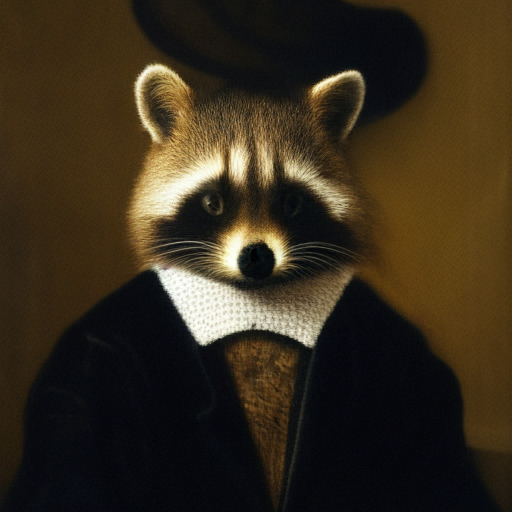
\includegraphics[width=50mm]{figs/verticals/style_00020_maskgit_sresg1r1} &
    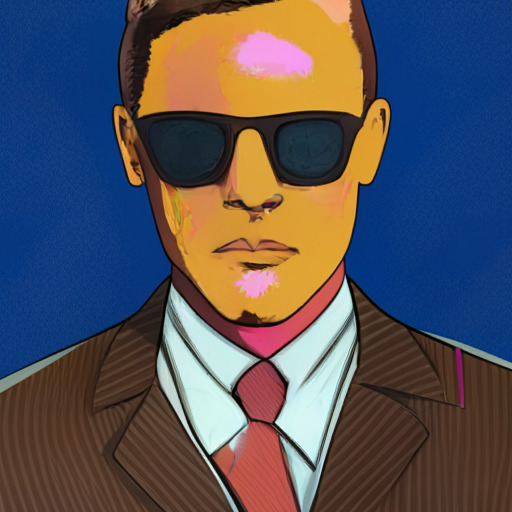
\includegraphics[width=50mm]{figs/verticals/style_00022_maskgit_sresg1r1} &
    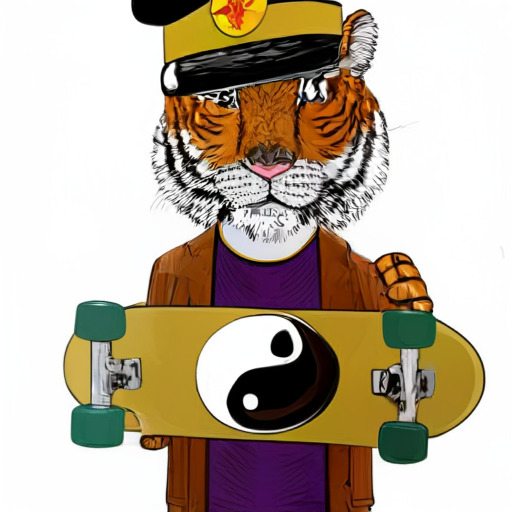
\includegraphics[width=50mm]{figs/verticals/style_01342_maskgit_sresg1r1}
    \\
    \small Portrait of a well-dressed raccoon, oil painting in the style of Rembrandt. &
    \small A portrait of a man wearing sunglasses and a business suit, painting in pop art style. &
    \small Portrait of a tiger wearing a train conductor's hat and holding a skateboard that has a yin-yang symbol on it. Chinese ink and wash painting.
    \\
  \end{tabular}
  \caption{Examples of text understanding in \name: \textbf{[top]} object cardinality is rendered correctly and in non-identical ways; \textbf{[middle]} multi-object compositionality (e.g., ``on'', ``left'', etc.) is rendered correctly; \textbf{[bottom]} artistic styles (e.g.,  ``oil painting'', ``pop art'', etc.) are rendered in a plausible manner.
\huiwen{let's move this figure to appendix, or website.}
}

  \label{fig:cardinality_composition_style_examples}
\end{figure}

\begin{figure}
  \centering
  \begin{tabular}{p{50mm}p{50mm}p{50mm}}
    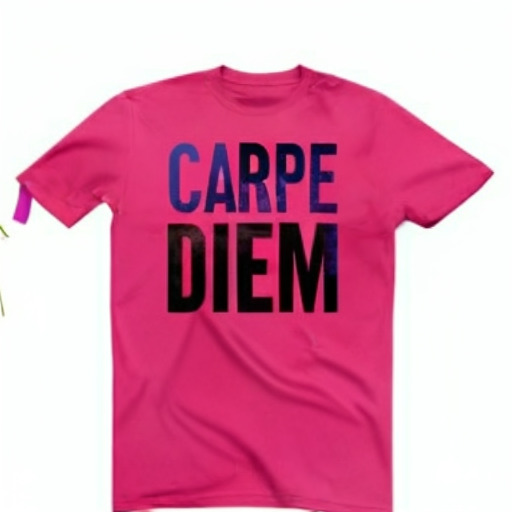
\includegraphics[width=50mm]{figs/verticals/text_00716_maskgit_sresg1r1} &
    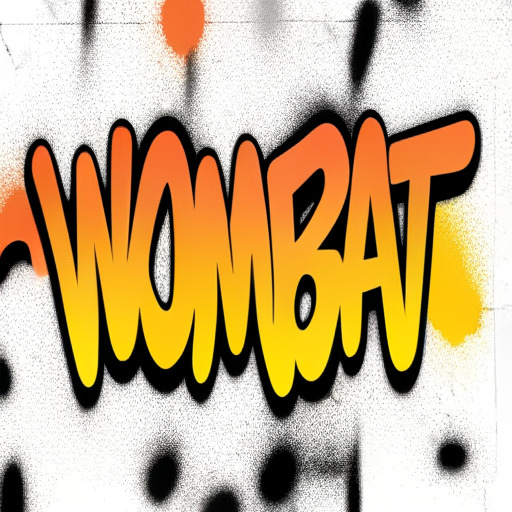
\includegraphics[width=50mm]{figs/verticals/text_01470_maskgit_sresg1r1} &
    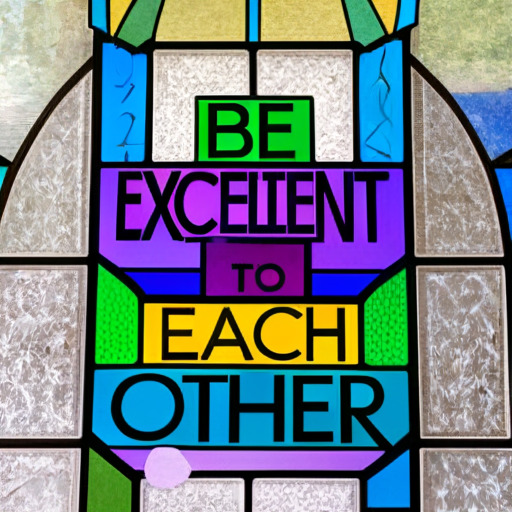
\includegraphics[width=50mm]{figs/verticals/text_01494_maskgit_sresg1r1}
    \\
    \small A t-shirt with Carpe Diem written on it. &
    %\small A motorcycle parked in an ornate bank lobby with ``BabelDraw'' written on its body. &
    \small High-contrast image of the word ``WOMBAT'' written with thick colored graffiti letters on a white wall with dramatic splashes of paint. &
    \small The saying ``BE EXCELLENT TO EACH OTHER'' written in a stained glass window.
    \\
    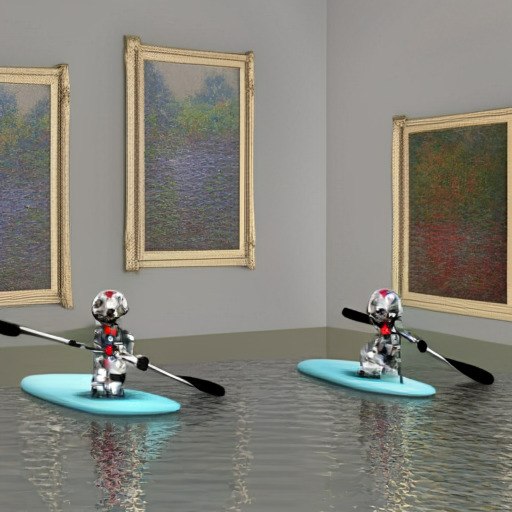
\includegraphics[width=50mm]{figs/verticals/detail_00030_maskgit_sresg1r1} &
    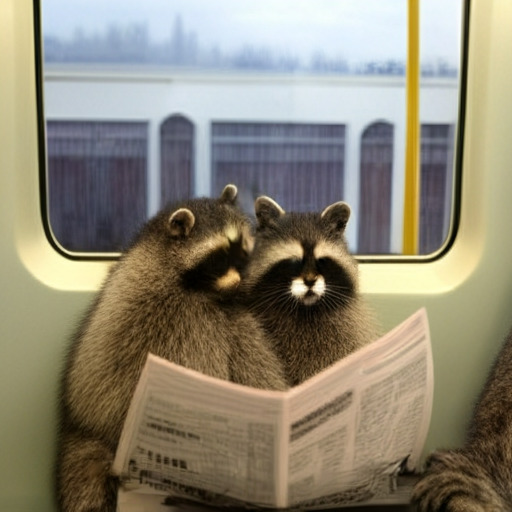
\includegraphics[width=50mm]{figs/verticals/detail_01370_maskgit_sresg1r1} &   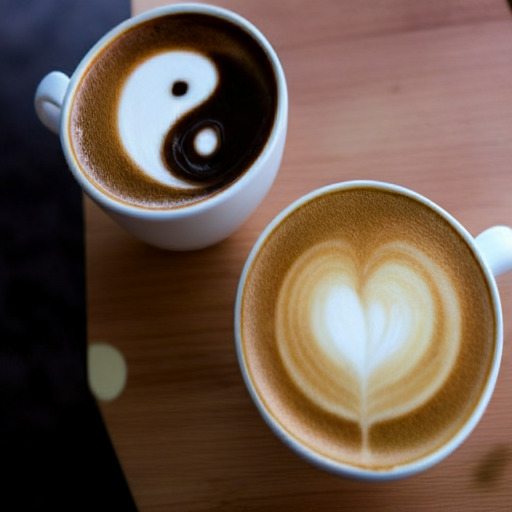
\includegraphics[width=50mm]{figs/verticals/detail_01459_maskgit_sresg1r1}
    %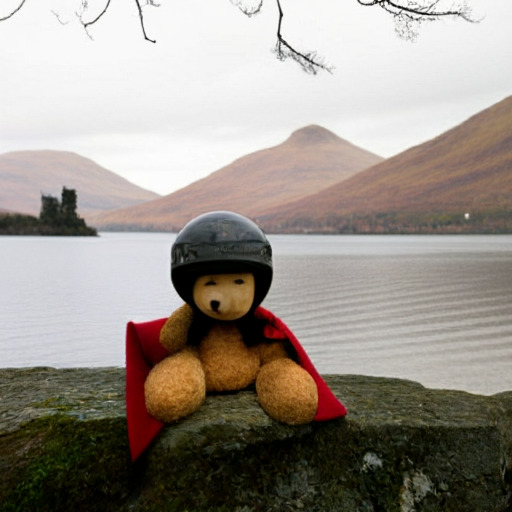
\includegraphics[width=50mm]{figs/verticals/detail_01577_maskgit_sresg1r1}
    \\
    \small An art gallery displaying Monet paintings. The art gallery is flooded. Robots are going around the art gallery using paddle boards. &
    \small A photograph of the inside of a subway train. There are raccoons sitting on the seats. One of them is reading a newspaper. The window shows the city in the background. &
    \small Two cups of coffee, one with latte art of yin yang symbol. The other has latter art of a heart.
    %\small A teddy bear wearing a motorcycle helmet and cape is standing in front of Loch Awe with Kilchurn Castle behind him. \\[6pt]

  \end{tabular}
  \caption{Examples of text understanding in \name: \textbf{[top]} text can be rendered accurately in many instances; \textbf{[bottom]} longer text prompts (up to $64$ tokens) are understood and generated appropriately.}
  \label{fig:word_and_indepth_examples}
\end{figure}

